\documentclass[xcolor=pdftex,table,10pt]{beamer}

\usetheme{default}
\usepackage[english]{babel}
\usepackage{graphicx}
\usepackage{verbatim}
\usepackage{listings}

\useoutertheme{infolines}
\useinnertheme{rectangles}

\graphicspath{{/home/za/Dokumen/idsecconf/2012/idsecconf2012/figure/}}

\begin{document}

\title{Pengujian Keamanan Aplikasi Mobile}
\subtitle{Studi Kasus: Android}
\author{Zaki Akhmad}
\institute{{\href{http://www.indocisc.co.id}{indocisc}}}
\date{10 Juni 2012}

\begin{frame}
	\titlepage
\end{frame}

\begin{frame}
	\frametitle{Tentang Zaki Akhmad}
		\begin{description}
			\item[Surel] za@indocisc.co.id 
			\item[Kunci Publik] 0xFD57BE80 di pgp.mit.edu
			\item[Twitter] @zakiakhmad	
			\item[indocisc] Analis, 2007 - sekarang
		\end{description}
	\begin{flushleft}
		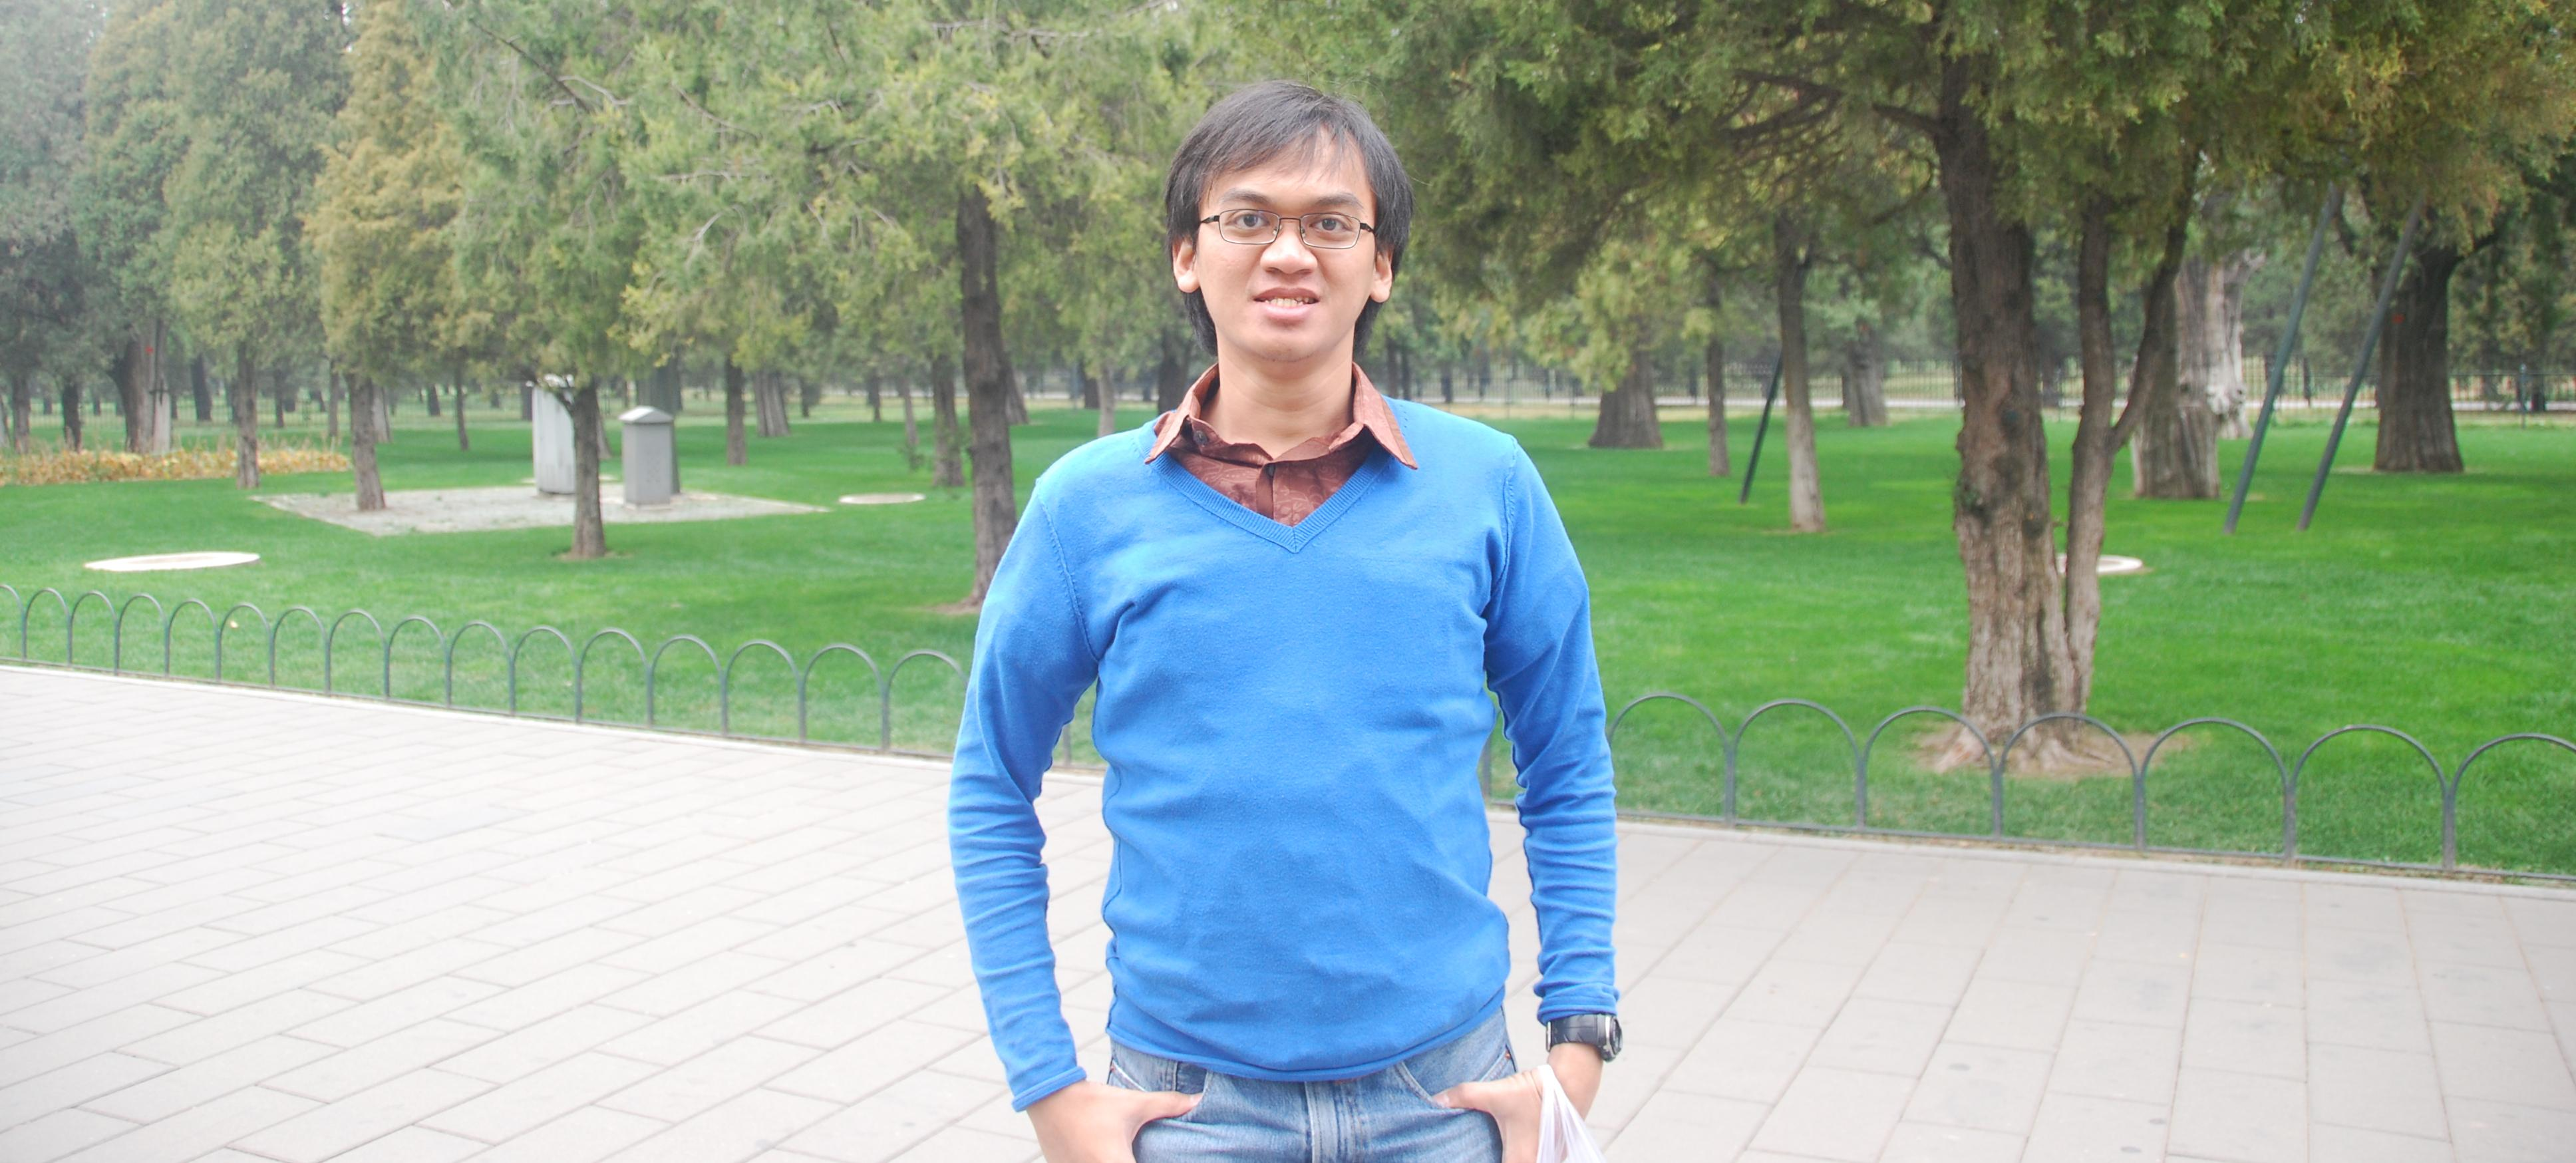
\includegraphics[height=3cm]{beijing.jpeg}
			\end{flushleft}
\end{frame}

\begin{frame}
	\begin{center}
		If you \textbf{fail} a penetration test \\ you know you have a very bad problem indeed. \\ If you \textbf{pass} a penetration test \\ you do not know that you don't have a very bad problem (Gary McGraw)
	\end{center}
\end{frame}

\begin{frame}
	\begin{center}
		\includegraphics<1>[height=5cm]{security-map.PNG}
		\includegraphics<2>[height=5cm]{gary-mcgraw.jpg}
		\includegraphics<3>[height=5cm]{ssdlc.PNG}
	\end{center}		
\end{frame}

\section*{Daftar Isi}

\begin{frame}
	\frametitle{Daftar Isi}
	\begin{columns}
	\column{0.4\textwidth}
		\tableofcontents
	\column{0.6\textwidth}
		\begin{center}
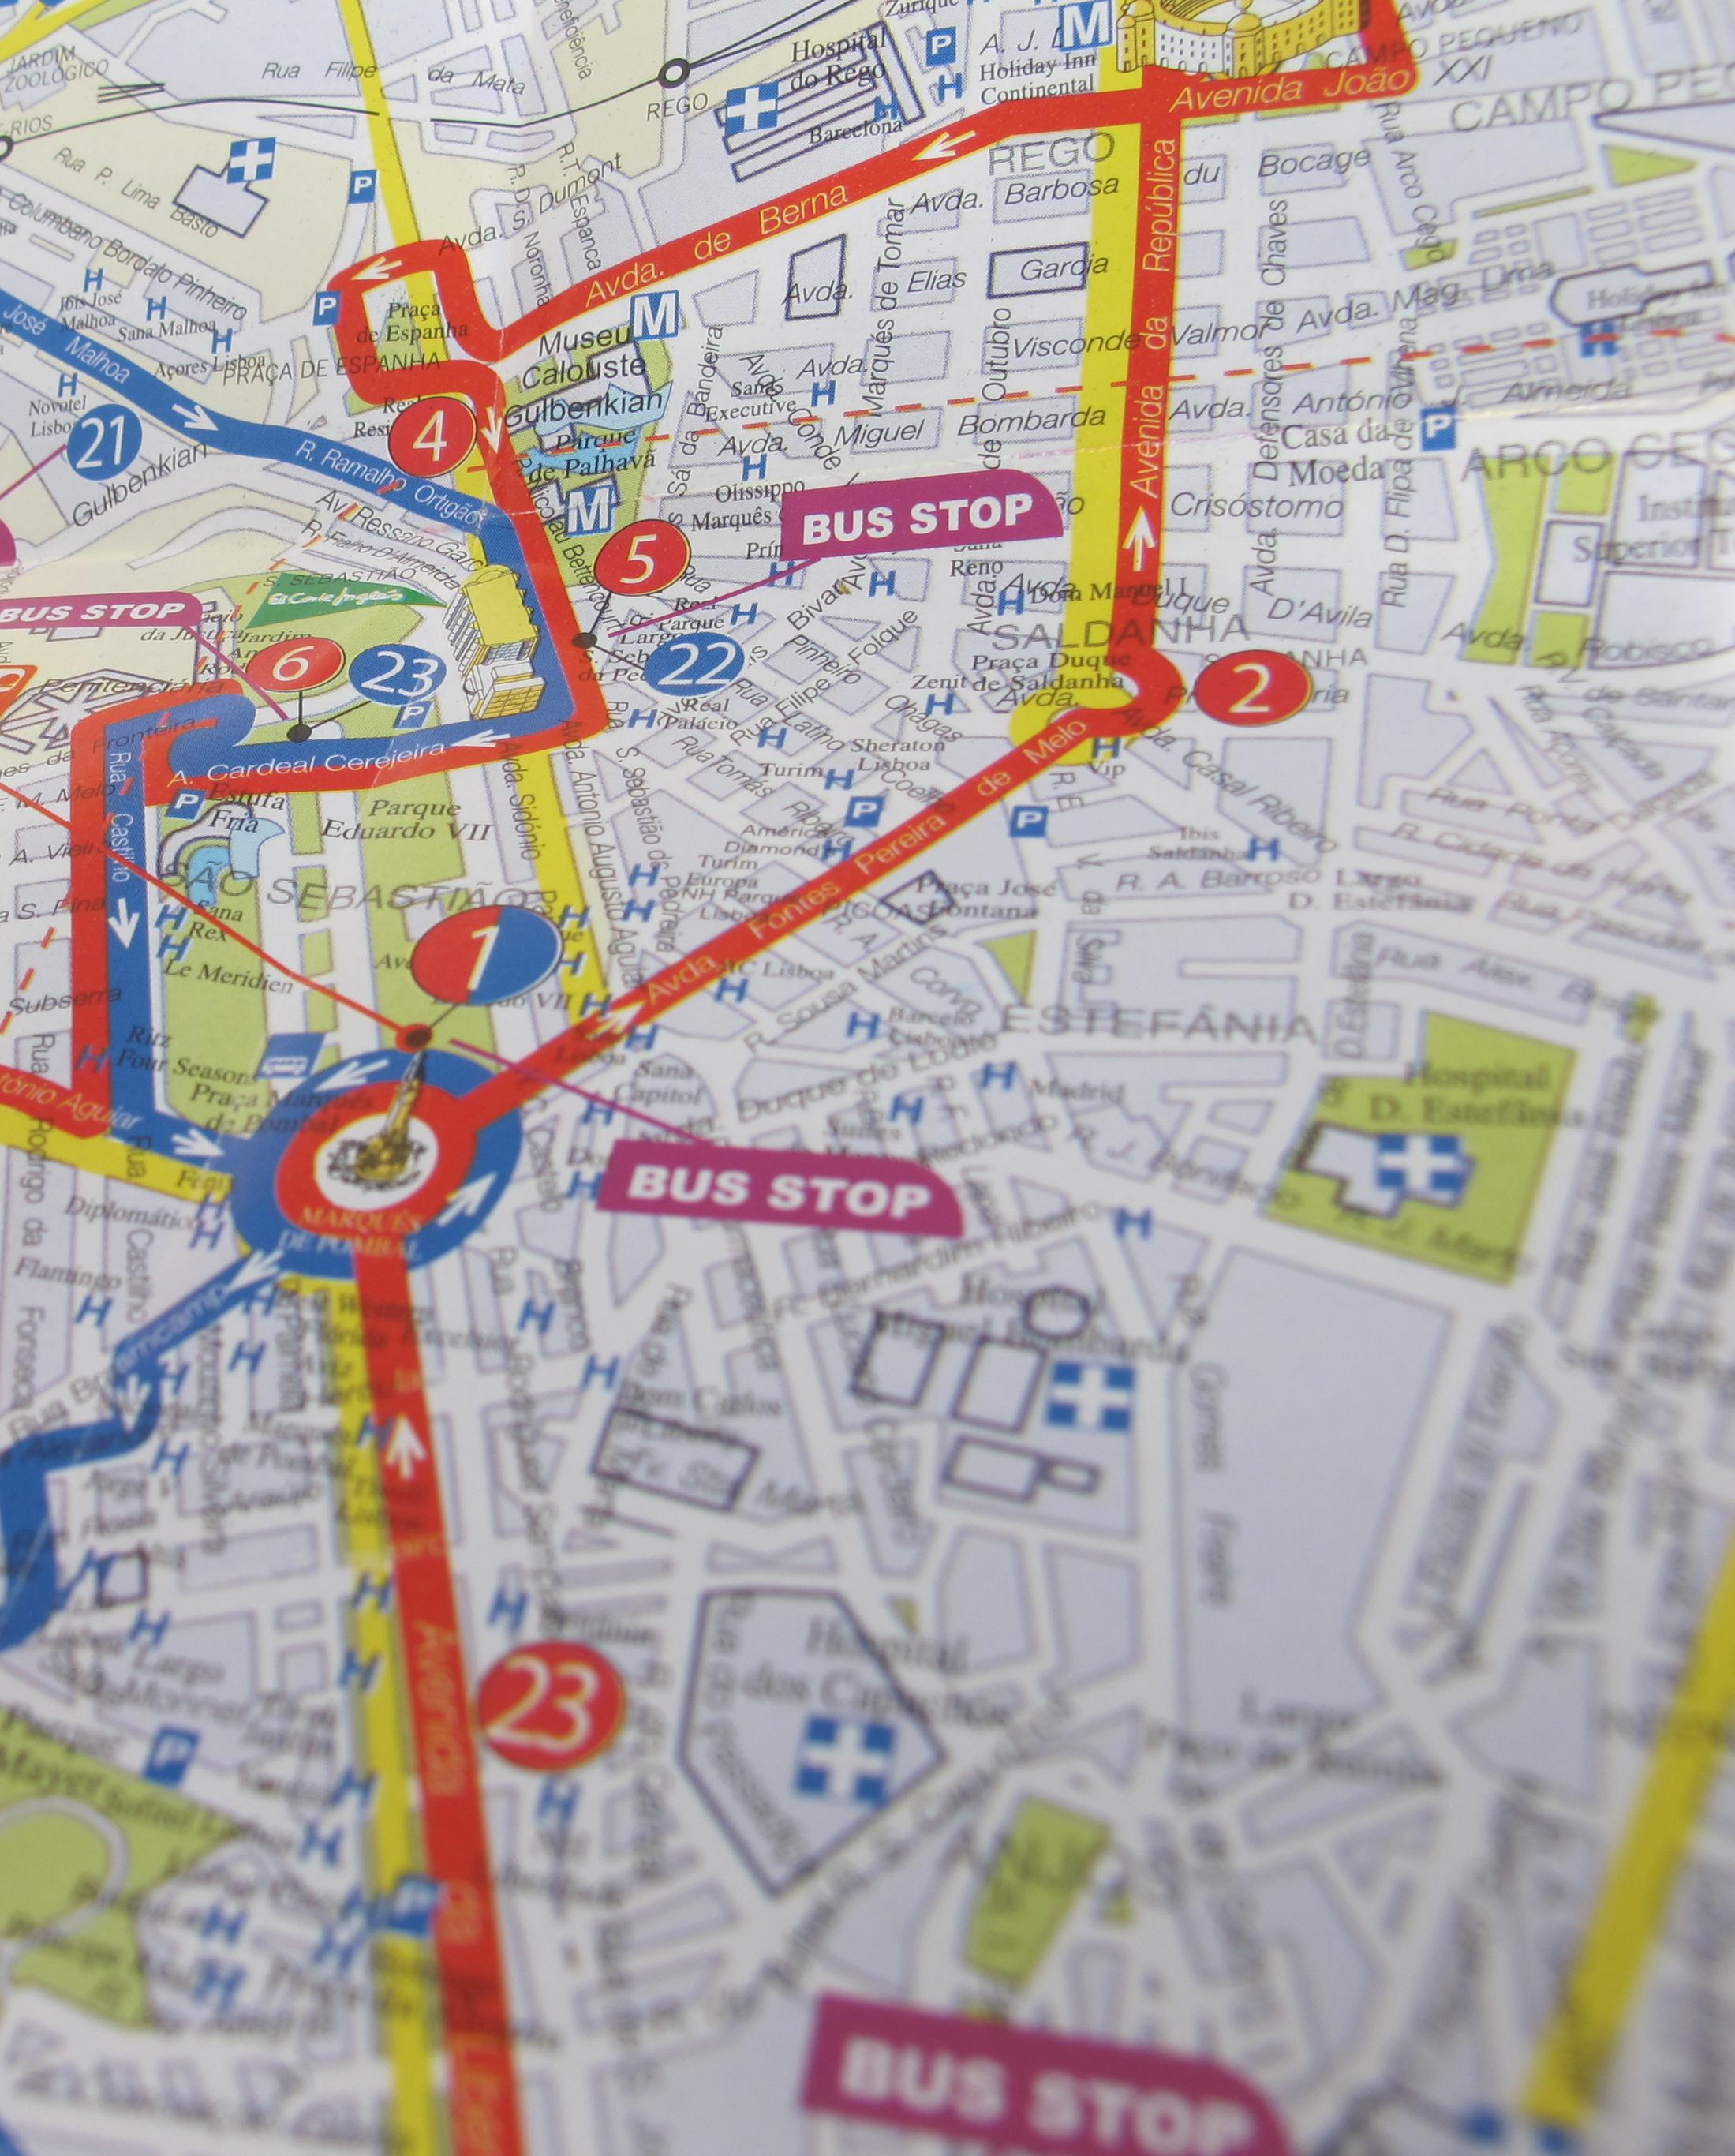
\includegraphics[height=5cm]{daftar-isi.jpeg}
\end{center}
	\end{columns}
\end{frame}

\section{Pengantar}
\begin{frame}
	\frametitle{Pengantar}
	\underline{Ponsel Pintar \textbf{Hanya} Sepintar Penggunanya}
	\begin{enumerate}
		\item Penggunaan di tempat umum
		\item Risiko hilang, siap?
		\item Aplikasi
		\begin{enumerate}
			\item Kecenderungan membuat \textit{password} yang sama
			\item Tidak tahu apakah menggunakan kanal terenkripsi/tidak
		\end{enumerate}
	\end{enumerate}
\end{frame}

\subsection{Konfigurasi Lab}
\begin{frame}
	\frametitle{Konfigurasi Lab}
	\underline{Langsung dari \textit{Device}} \vskip1.5cm
	\begin{center}
\texttt{komputer -> kabel data - > ponsel}
\end{center}
\end{frame}

\begin{frame}
	\frametitle{Konfigurasi Lab}
	\underline{Menggunakan Hub} \vskip1.5cm
	\begin{center}
\texttt{ponsel -> hub - > Komputer:Internet}
\end{center}
\end{frame}


\begin{frame}
	\frametitle{Konfigurasi Lab}
	\underline{Menggunakan Emulator}
	\begin{center}
		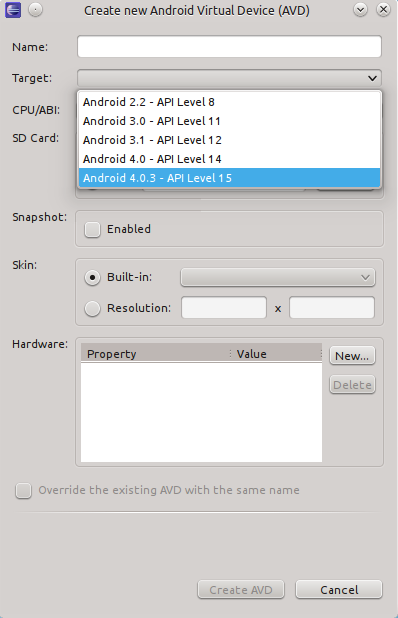
\includegraphics[height=6cm]{03_AVD.png}
	\end{center}
\end{frame}


\section{Teori Pengujian}

\begin{frame}
	\frametitle{Dinamis vs Statis}
	\begin{columns}	
	\column{.5\textwidth}
		\begin{flushright} 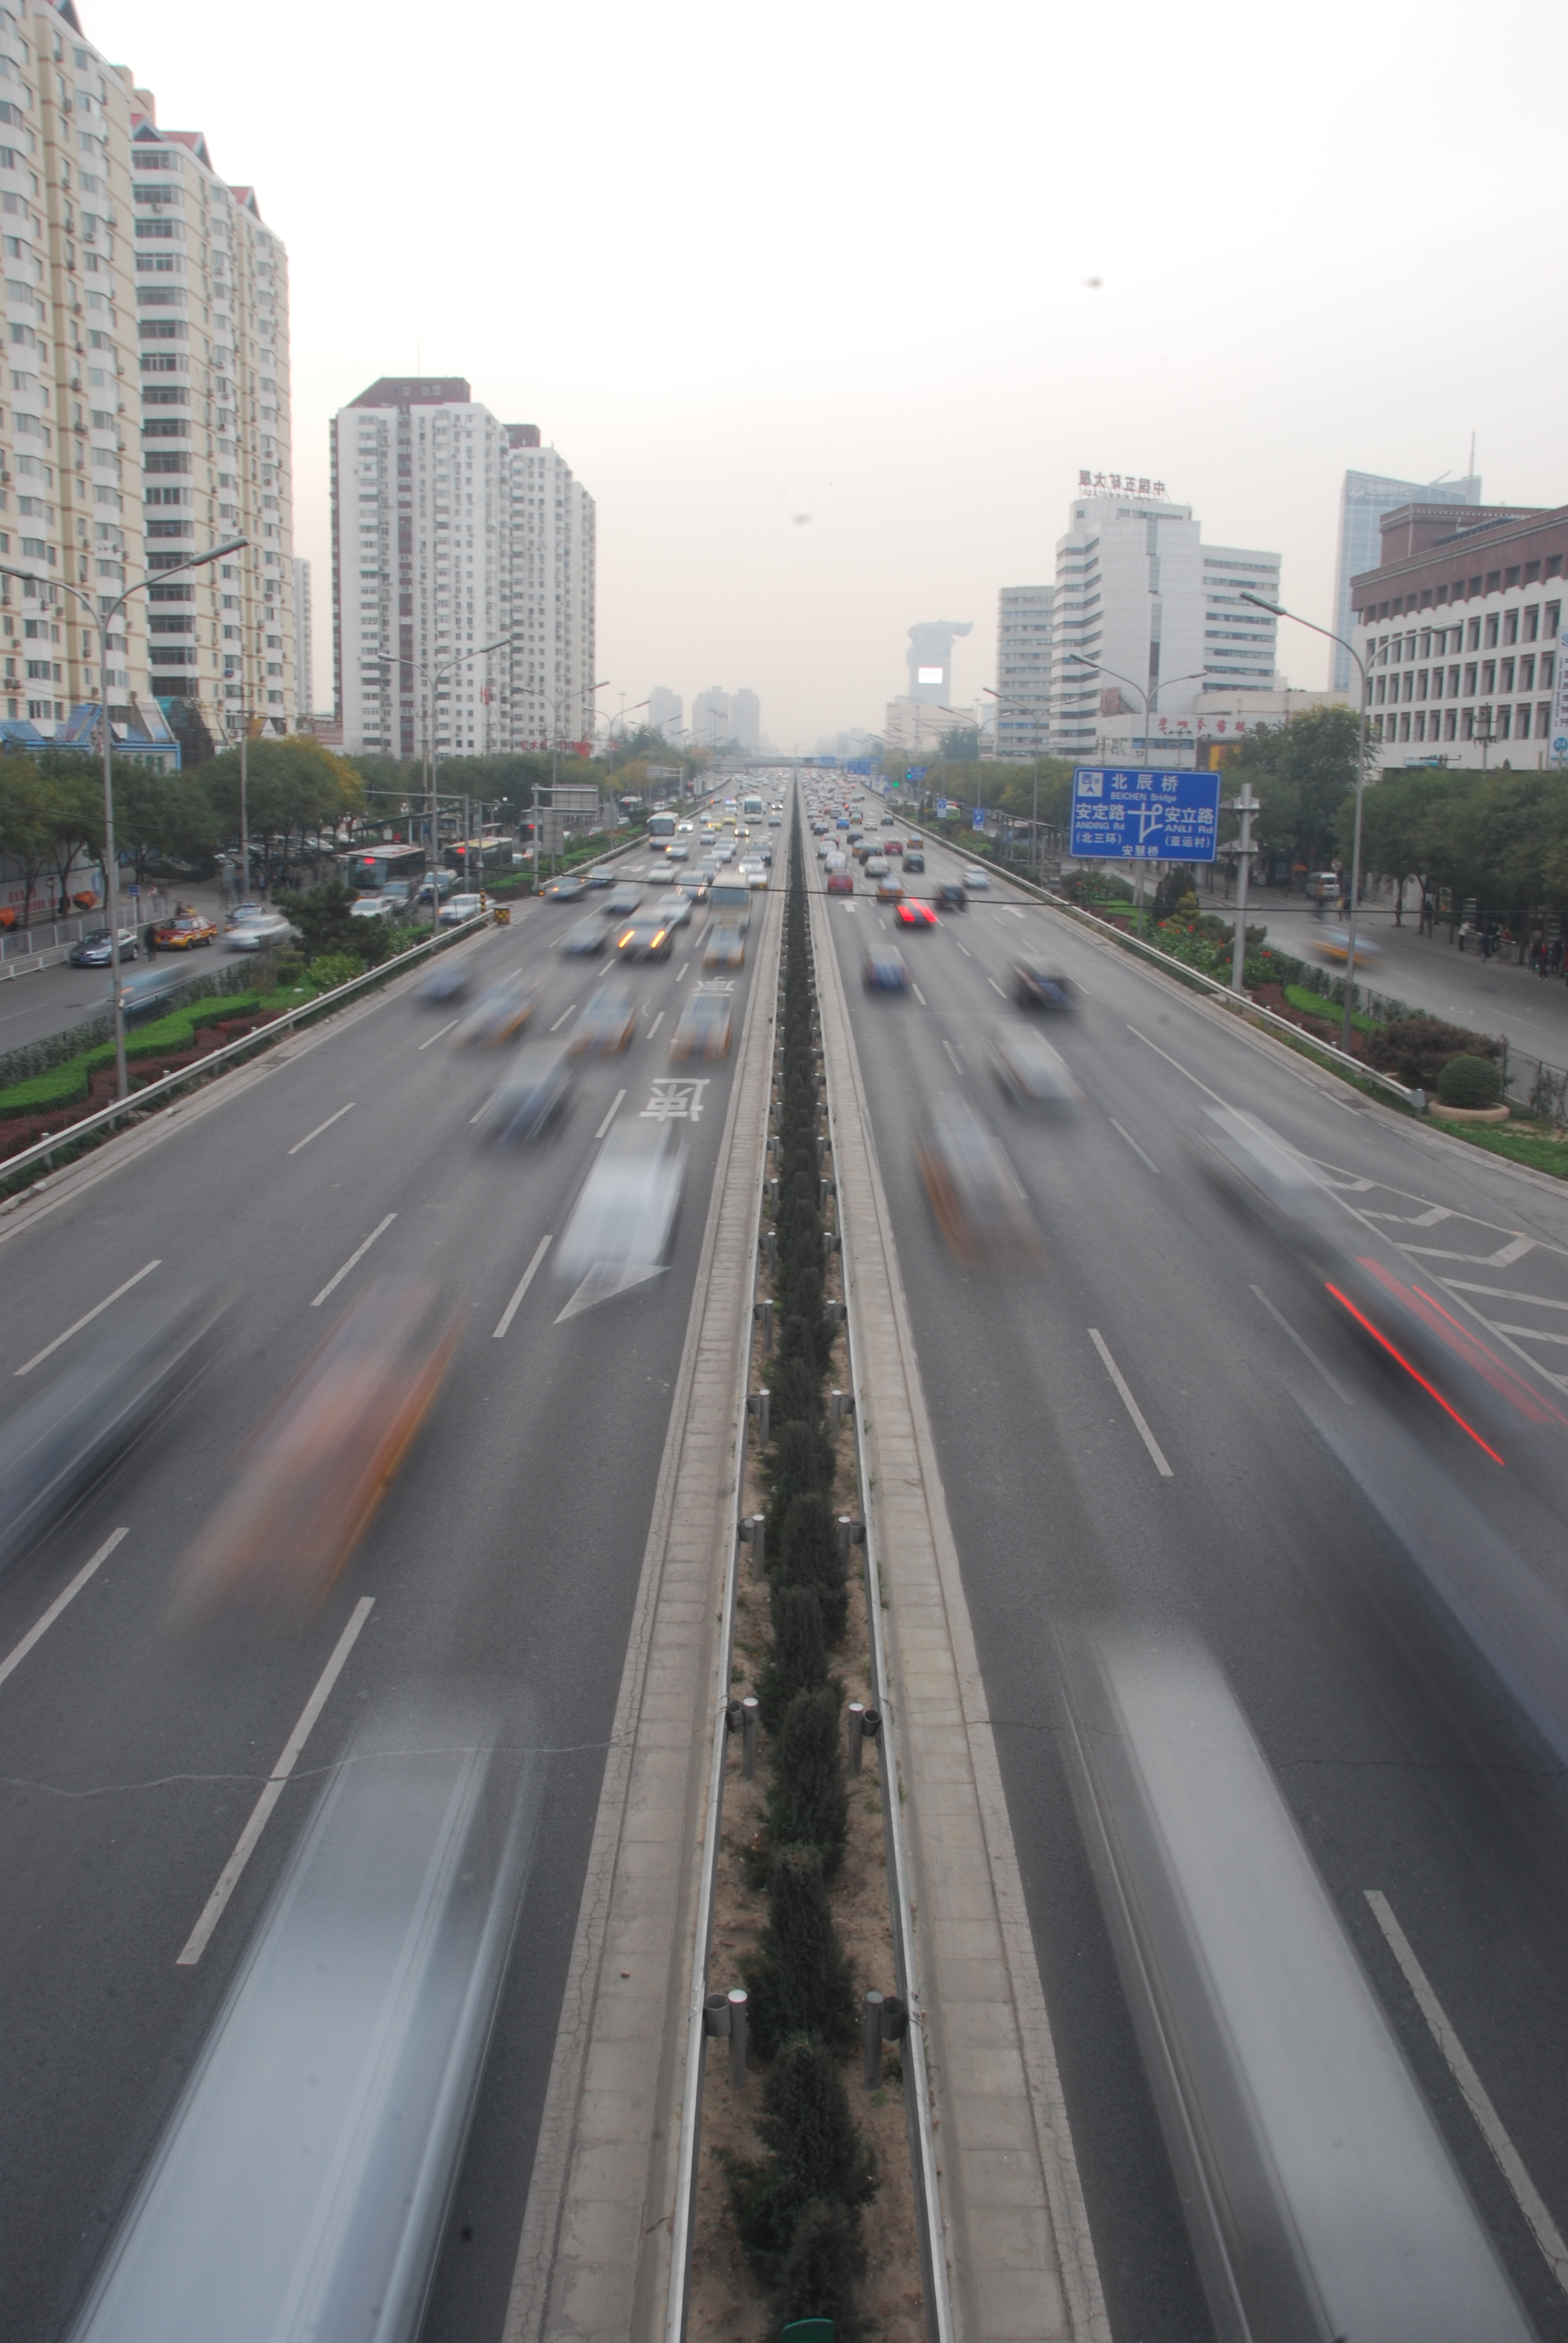
\includegraphics[height=4.5cm]{dynamic.jpg} \end{flushright}
	\column{.5\textwidth}
		\begin{flushleft}
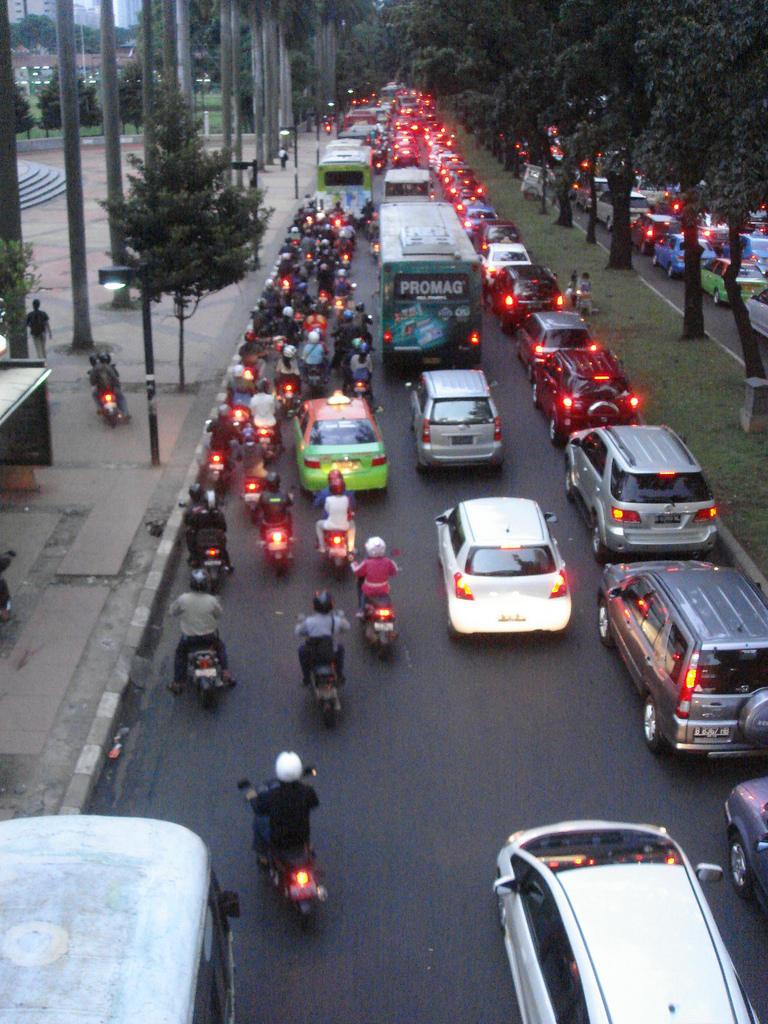
\includegraphics[height=4.5cm]{static.jpeg}
\end{flushleft}
	\end{columns}
\end{frame}

\subsection{Pengujian Dinamis}
\begin{frame}
	\frametitle{Pengujian Dinamis}
	Pengujian dinamis adalah pengujian yang dilakukan \textbf{dengan} menjalankan aplikasi 
	\begin{enumerate}
		\item Analisis \textit{network traffic}
		\item Analisis \textit{remote services} (HTTP/SOAP/dll)
		\item Debug aplikasi
	\end{enumerate}
\end{frame}

\subsection{Pengujian Statis}
\begin{frame}
	\frametitle{Pengujian Statis}
	Pengujian statis adalah pengujian yang dilakukan \textbf{tanpa} menjalankan aplikasi 	
	\begin{enumerate}
		\item Dapatkan aplikasi
		\begin{enumerate}
			\item Ekstrak aplikasi dari device
			\item Dapatkan berkas installer dari pengembang
		\end{enumerate}				
		\item Lakukan \textit{reverse engineering}
		\item Lakukan \textit{source code review}
	\end{enumerate}
\end{frame}

\section{Hasil Pengujian}

\subsection{Wordpress}
\subsubsection{Dinamis}

\begin{frame}
	\frametitle{Pengujian Dinamis Aplikasi Wordpress}
	\begin{itemize}
		\item Analisis \textit{Network Traffic} \\
		Aktivitas yang dilakukan:
		\begin{itemize}
			\item Akses sebagai publik (tanpa otentikasi)
			\item Melakukan otentikasi, masuk sebagai \textit{authorized user}
			\item Menulis tulisan baru
			\item Akses menu Wordpress
			\item Mengubah password
		\end{itemize}
		\item Debug Aplikasi
	\end{itemize}
\end{frame}

\begin{frame}
	\frametitle{Pengujian Dinamis Aplikasi Wordpress}
	\underline{Analisis \textit{Network Traffic}}	
	\begin{center}
	\includegraphics<1>[height=5cm]{04_wpandroid-post.png} 
	\includegraphics<2>[height=5cm]{05_wpandroid-newPost-1.png} 
	\includegraphics<3>[height=5cm]{06_wpandroid-changepassword.png} 
	\includegraphics<4>[height=5cm]{07_SC20120420-103832.png} 
\end{center}
	
\end{frame}

\begin{frame}
	\frametitle{Pengujian Dinamis Aplikasi Wordpress}
	\underline{Debug Aplikasi} \\
	Mencari informasi sensitif yang tersimpan dalam device
	\begin{enumerate}
		\item List device menggunakan \texttt{adb}
		\item Masuk ke \texttt{shell}
		\item Cari direktori database aplikasi
		\item Gunakan perintah \texttt{dump} untuk melihat isi database
	\end{enumerate}
\end{frame}

\subsubsection{Statis}
\begin{frame}
	\frametitle{Pengujian Statis Aplikasi Wordpress}
	\begin{center}
		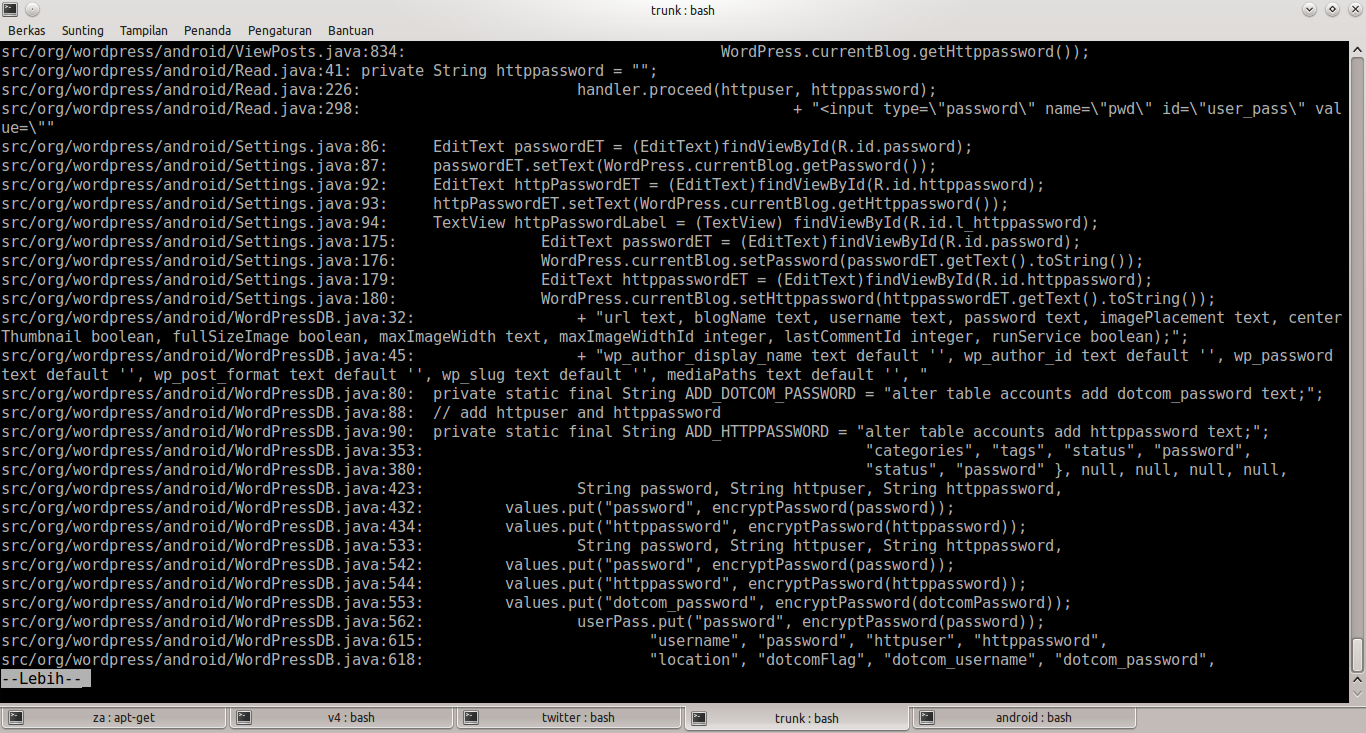
\includegraphics[height=5cm]{17_wordpress-password-src.png} \\
		Mencari kata \texttt{password}
	\end{center}
\end{frame}

\subsection{Twitter}
\subsubsection{Dinamis}

\begin{frame}
	\frametitle{Pengujian Dinamis Aplikasi Twitter}
	\begin{itemize}
		\item Analisis \textit{Network Traffic} \\
		Aktivitas yang dilakukan:
		\begin{itemize}
			\item Install aplikasi Twitter untuk Android dari Google Play
			\item Jalankan kali pertama
			\item Login
			\item Twit
		\end{itemize}	
		\item Debug Aplikasi	 
	\end{itemize}
\end{frame}

\begin{frame}
	\frametitle{Pengujian Dinamis Aplikasi Twitter}
	\underline{Analisis \textit{Network Traffic}}
	\begin{center}
		\includegraphics<1>[height=4cm]{09_twitter-googleplay.png}
		\includegraphics<2>[height=4cm]{10_twitter-response-manifest.png}
		\includegraphics<3>[height=4cm]{11_twitter-reassemble.png}
		\includegraphics<4>[height=4cm]{12_twitter-get-image.png}
		\includegraphics<5>[height=4cm]{13_twitter-application-data.png}
	\end{center}
\end{frame}


\begin{frame}
	\frametitle{Pengujian Dinamis Aplikasi Twitter}
	\underline{Debug Aplikasi} \\
	Mencari informasi sensitif yang tersimpan dalam device
	\begin{enumerate}
		\item Dapatkan file \texttt{.apk} Twitter untuk Android
		\item Install aplikasi pada emulator
		\item Cari direktori database
		\item Dump database
	\end{enumerate}
\end{frame}

\begin{frame}
	\frametitle{Pengujian Dinamis Aplikasi Twitter}
	\begin{center}
		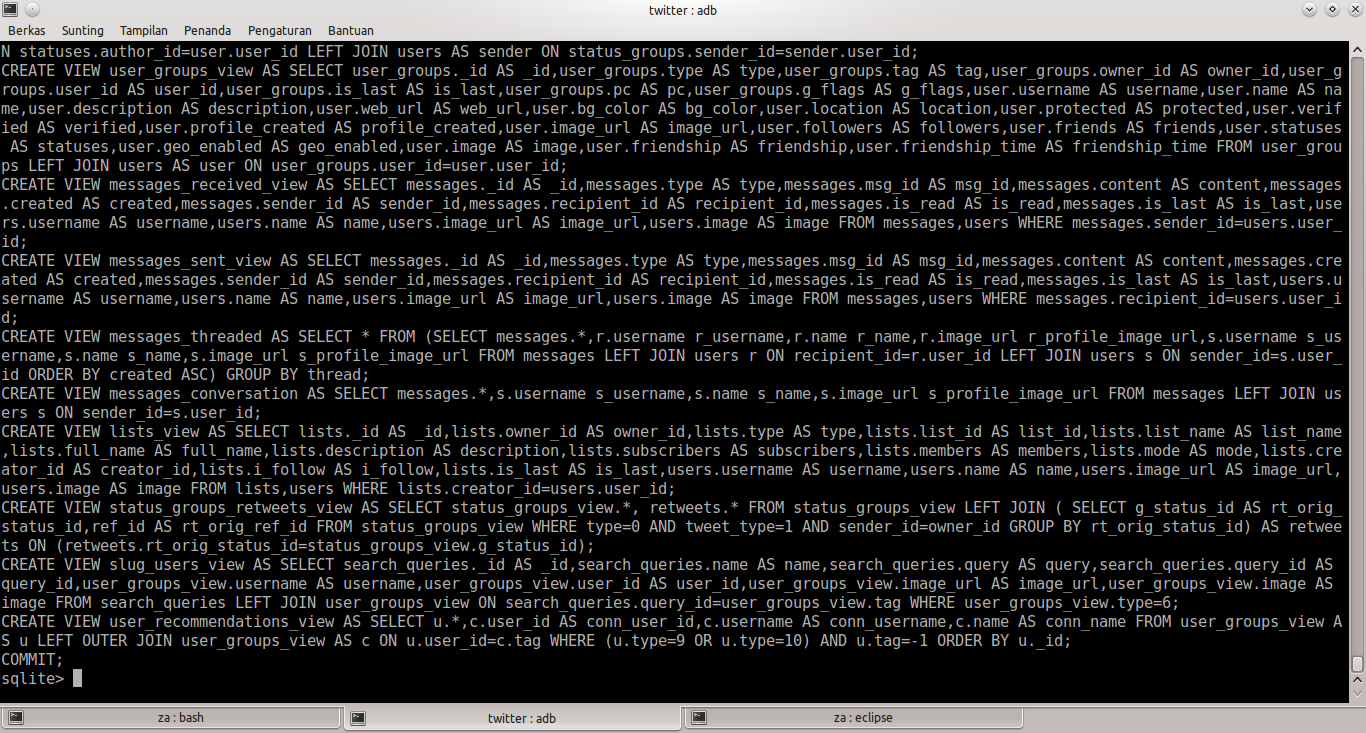
\includegraphics[height=5cm]{16_twitter-dump-15016157.png} \\
		Dump database twitter
	\end{center}
\end{frame}

\subsubsection{Statis}
\begin{frame}
	\frametitle{Pengujian Statis Aplikasi Twitter}
	\underline{Lakukan \textit{reverse engineering}}	
	\begin{enumerate}
		\item \texttt{unzip twitter.apk}
		\item Gunakan \texttt{apk tool} untuk mendapatkan berkas \texttt{AndroidManifest.xml} dalam format \textit{plain text}.
		\item Analisis berkas \texttt{AndroidManifest.xml}		
	\end{enumerate}		
\end{frame}

\begin{frame}
	\frametitle{Pengujian Statis Aplikasi Twitter}
	\begin{center}	
	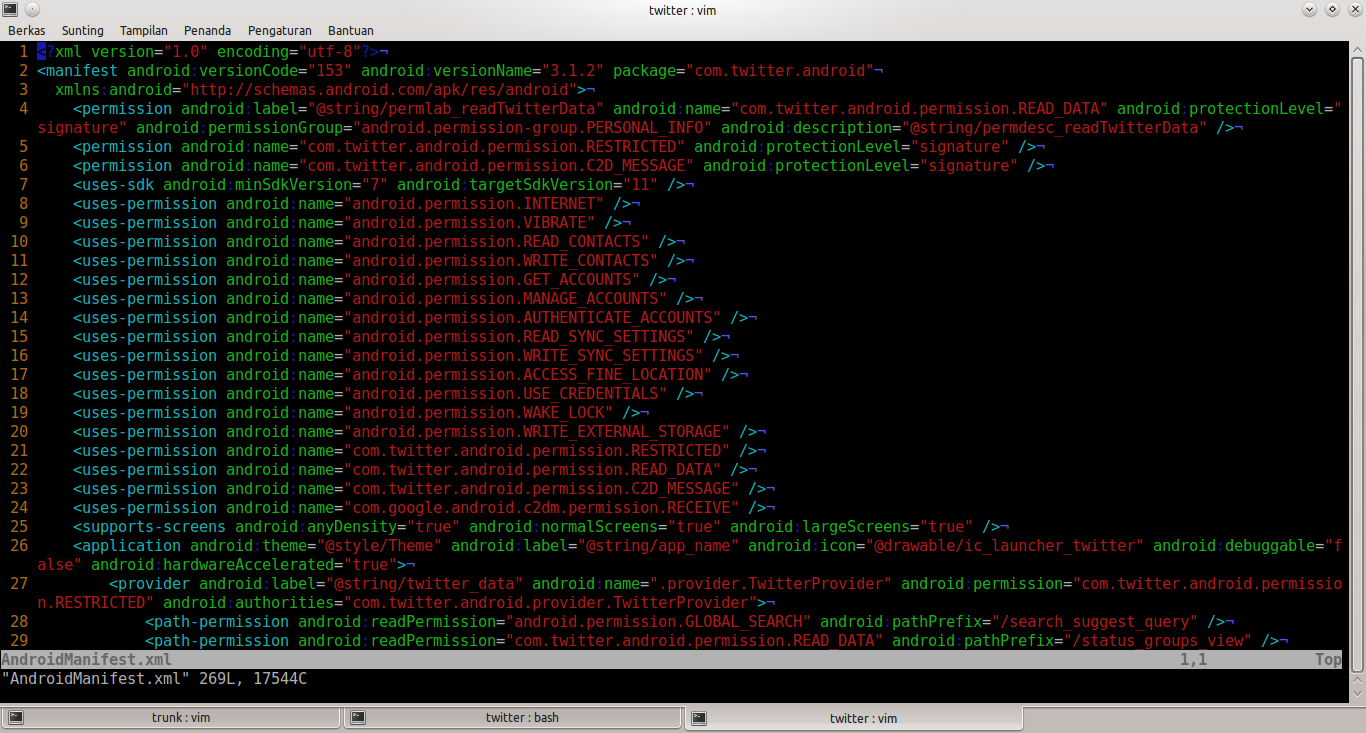
\includegraphics[height=5cm]{19_twitter-androidmanifest.png} \\
	Berkas \texttt{AndroidManifest.xml} Twitter
	\end{center}
\end{frame}

\section{Penutup}
\subsection{Kesimpulan dan Saran}
\begin{frame}
	\frametitle{Kesimpulan}
	\underline{Kesimpulan} \\
	\begin{enumerate}
		\item Wordpress untuk Android
		\begin{enumerate}
			\item Setiap melakukan request, UserID dan Password dikirim dalam keadaan clear text. 
			\item UserID dan password tersimpan dalam database dalam format clear text. 
		\end{enumerate}
		\item Twitter untuk Android
		\begin{enumerate}
			\item Menggunakan transport layer terenkripsi saat mengakses server
			\item UserID dan password tersimpan dalam keadaan terenkripsi
			\item Direct message tersimpan dalam format clear text
		\end{enumerate}
	\end{enumerate}

\end{frame}

\begin{frame}
	\frametitle{Saran}
	\underline{Saran}	
	\begin{enumerate}
		\item Pada pengujian dinamis, lakukan \textit{intercept traffic} antara aplikasi dengan server menggunakan \textit{proxy} sehingga dapat dilakukan analisis lebih mendalam
		\item Pada pengujian statis, pelajari lebih detail bagaimana mengembangkan aplikasi Android (atau aplikasi mobile pada umumnya) sehingga dapat melakukan \textit{code review} lebih baik
	\end{enumerate}
\end{frame}

\begin{comment}
\subsection{Ringkasan}
\begin{frame}
	\frametitle{Ringkasan}
\end{frame}
\end{comment}

\section{Referensi}
\begin{frame}
	 \frametitle{Referensi}
	\begin{itemize}	
		\item {\href{http://code.google.com/p/android-apktool}{APK-Tool}}
		\item {\href{http://jack-mannino.blogspot.com/2010/09/reversing-android-apps-101.html}{Jack Maninno, Reversing Android Apps 101}}			
		\item {\href{http://www.amazon.com/Application-Security-Android-Platform-Permissions/dp/1449315070}{Jeff Six, Application Security for the Android Platform, O'Reilly}}
		\item {\href{https://www.owasp.org/index.php/OWASP_Mobile_Security_Project}{OWASP Mobile Security Project}}
		\item {\href{http://developer.android.com}{Situs Pengembang Android}}	
		\item {\href{https://dev.twitter.com}{Situs Pengembang Twitter}}
		\item {\href{http://dev.android.wordpress.org/}{Situs Pengembang Wordpress}}	
	\end{itemize}
\end{frame}

\begin{frame}
	\frametitle{Terima Kasih}
	\begin{center}
		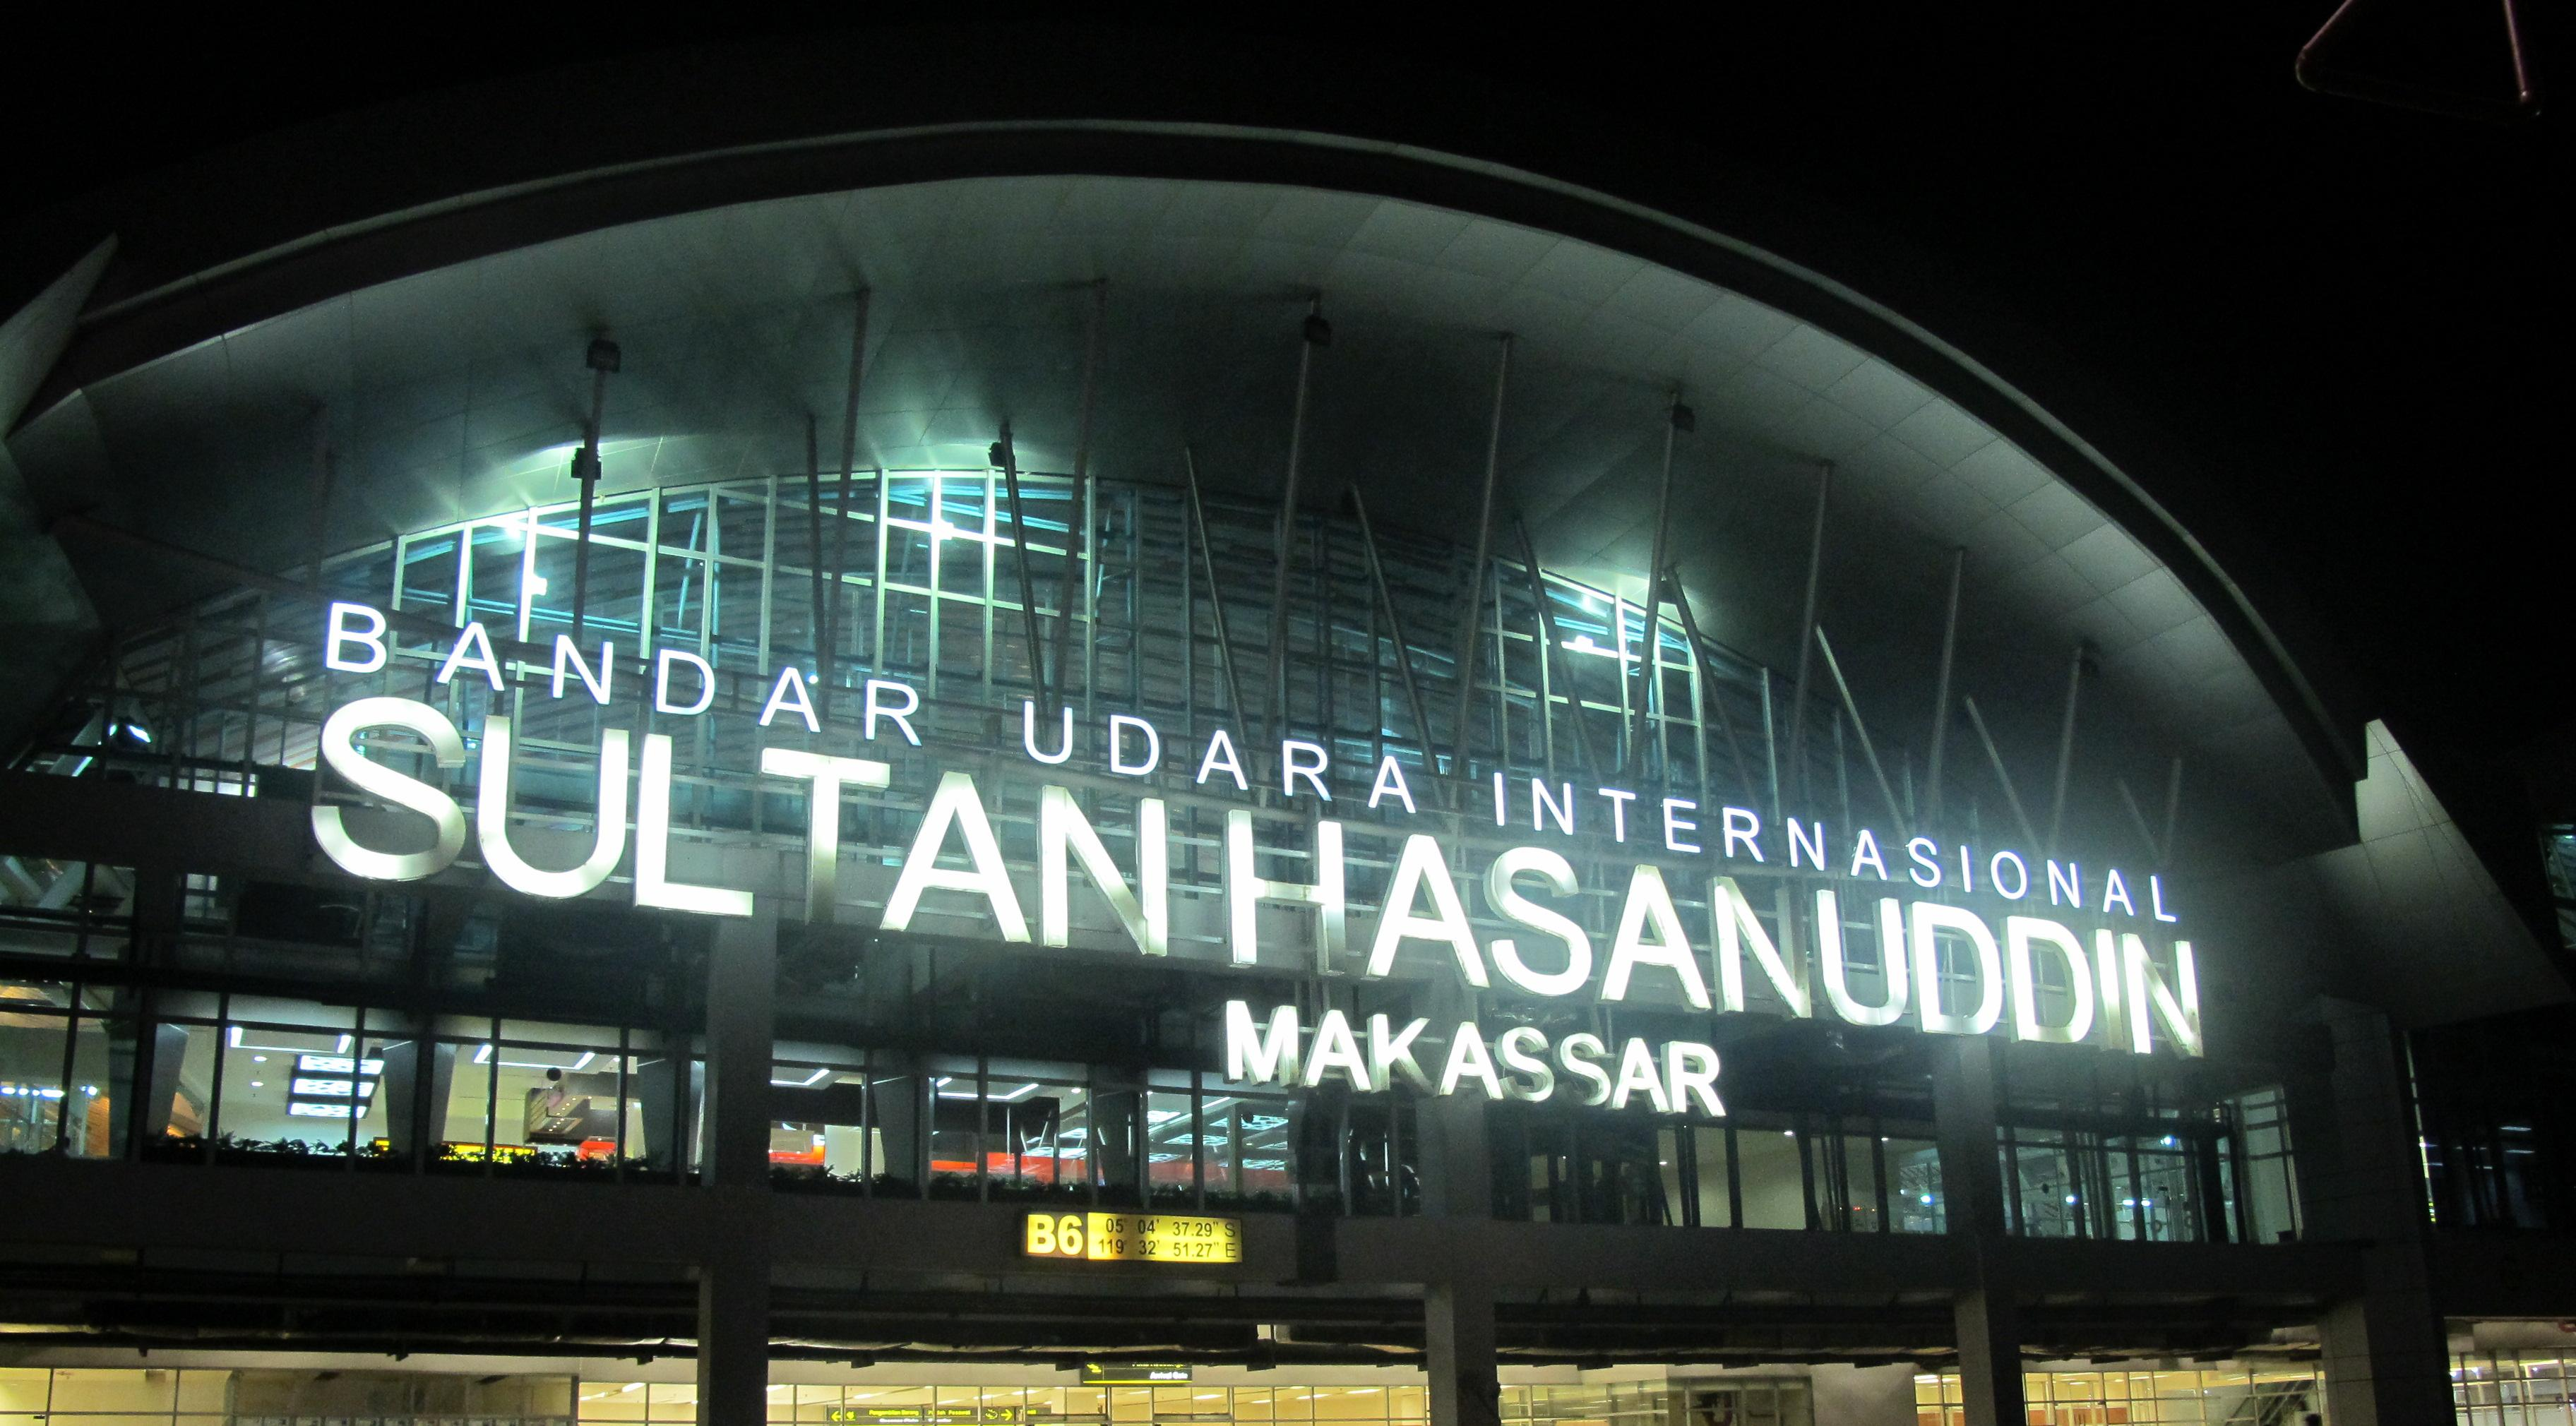
\includegraphics[height=5cm]{mks-bandara.JPG}
		\vskip.5cm \textit{kurru sumanga \\ thank you, arigatou, danke, merci beaucoup \\}
		\vskip.3cm		
		\tiny{foto-foto {\href{http://flickr.com/zakiakhmad}{flickr.com/zakiakhmad}}}
	\end{center}	
	
\end{frame}

\end{document}
